\section{Station Centrality}

Network centrality is a measure of the importance of a given node to a network. Central nodes need not be at the geometric center of a network map, indeed certain networks wont have a geometric center. The centrality of a given node can be computed relative to position, relative to adjacency, or relative to flow. A computationally simple way to compute adjacency-focused centrality is degree centrality. Degree centrality is defined as

\begin{equation}
	\Omega_d(v) = \frac{\eta(v)}{n - 1}
\end{equation}

where $\eta(v)$ is a function returning a value computed from the adjacency of node $v$. Degree is the number of adjacent nodes adjacent to a given node. Nodes of high degree will often be important to a network but are not necessarily so. As an example, several major US freeways meet in the greater Los Angeles area and service a huge amount of traffic to and from the area. Los Angeles thus has high valency with respect to the US freeway network. However, it is intuitive to note that Los Angeles is not central to the US freeway network being located at a near fringe. Were the freeways in Los Angeles to be shut down performance across the network would be less effected than it would be for the loss of Denver, Kansas City, Oklahoma City, or St. Louis even though Los Angeles is more populated and produces more traffic than any of those mentioned cities. Because of Los Angeles's geographic location, relatively little traffic will flow through it from other origins to other destinations. Thus Los Angeles has relatively low flow centrality. Fundamentally, the reason that degree centrality is misleading for the US freeway network is that its nodes are spatially defined. Indeed, the US transportation network would be more efficient if high-traffic-generation nodes like Los Angeles were located in its geometric center. For networks wherein nodes can be moved or node capacity can be changed (such as logistics networks) over time degree centrality will come to approximate flow centrality.

Flow centrality requires an estimation of network traffic at a node level. To compute traffic, one generally needs to compute lowest-cost paths. Suppose that for a graph $G$, the sets of shortest paths from each node $v$ to all other nodes $R_{v,U}$ and vice versa $R_{U,v}$ are known. From the optimal routes betweenness centrality and closeness centrality can be computed.

Betweenness centrality is defined as

\begin{equation}
	\Omega_b(v) = \sum_{o, d \in V}\frac{\sigma(o, d\ |\ v)}{\sigma(o, d)}\label{eq:betweenness_centrality}
\end{equation}

where $\sigma(o, d\ |\ v)$ is the weighted sum of the set of shortest paths between $o$ and $d$ which contain $v$ and $\sigma(o, d)$ is the weighted sum of the set of shortest paths between $o$ and $d$. Betweenness centrality reflects the relative volume of use for a node in a graph (and may also be computed for edges). Returning to the US freeway system, since very few O/D pairs would feature shortest paths through Los Angeles, the betweenness centrality of Los Angeles would be appropriately low. However, if weighted by O/D traffic volume, Los Angeles's centrality may be inflated. Another way to look at centrality is closeness centrality defined as

\begin{equation}
	\Omega_c(v) = \frac{n - 1}{\sum_{u \in U} \eta(v, u)}
\end{equation}

where $n$ is the cardinality of $V$ and $\eta(v, u)$ is the cost of the shortest path from $v$ to $u$. For the US freeway network cities like Denver and St. Louis will have high closeness centrality where Los Angeles will have low closeness centrality. The flow based measures of centrality model centrality on the basis of network behavior as observed. Both flow based measures could be applied to networks on the basis of recorded traffic rather than computed shortest paths. In other words, flow-based centrality measures only relate to network structure to the extent that observed traffic is determined by network structure. Flow-based centrality measures are perfect information metrics.

In reality, particularly with respect to transportation, information is imperfect. What this means in practice is that individual drivers have many options for each O/D pair and will not necessarily pick the shortest path. Furthermore, many paths may share edges or sequences of edged and, for much of the route, the remaining route will be uncertain even if the O/D pair is known. As one progresses along a route information will increase and entropy will decrease but this will not be a linear relationship. Certain nodes will be much more determinative than others. A practical example is the decision to merge onto a freeway. Once a driver merges onto a freeway it is very likely that the driver will stay on freeways until close until the destination. On the other hand, when traversing a street grid diagonally no action is particularly determinative over future actions. Information centrality measures the inverse of the information gained upon reaching a given node on the theory that the most central nodes provide the most options. Information centrality for the nodes in $G = \{V, E\}$ is based on the inverse incidence matrix $B$ whose elements are

\begin{align}
	b_{ij} = \begin{cases}
		1 & (i, j) \not\in E \\
		1 - \eta(i, j) & (i, j) \in E
	\end{cases}\quad i\neq j \\
	b_{ii} = 1 + \sum_{(i, j) \in E_i} \eta(i, j)
\end{align}

where $\eta(i, j)$ is a function returning edge costs. The diagonal elements of $B$ are the degrees of $V$ plus self-connection and the non-diagonal elements are 1 if no direct connection exists and less than 1 where one does exist. Rows and columns of $B$ all have the same sum if $G$ is reciprocal. The information for each node can be computed form the incidence matrix $C = D^{-1}$ as

\begin{equation}
	\Omega_i(v) = \frac{n}{nc_{vv} + \sum_{u = 1}^{n} c_{uu} - 2 \sum_{u = 1}^{n}c_{vu}}\label{eq:information_centrality}
\end{equation}

The methods of computing centrality are compared for the simple graph shown in Figure \ref{fig:simple_graph}.

\begin{figure}[H]
	\centering
	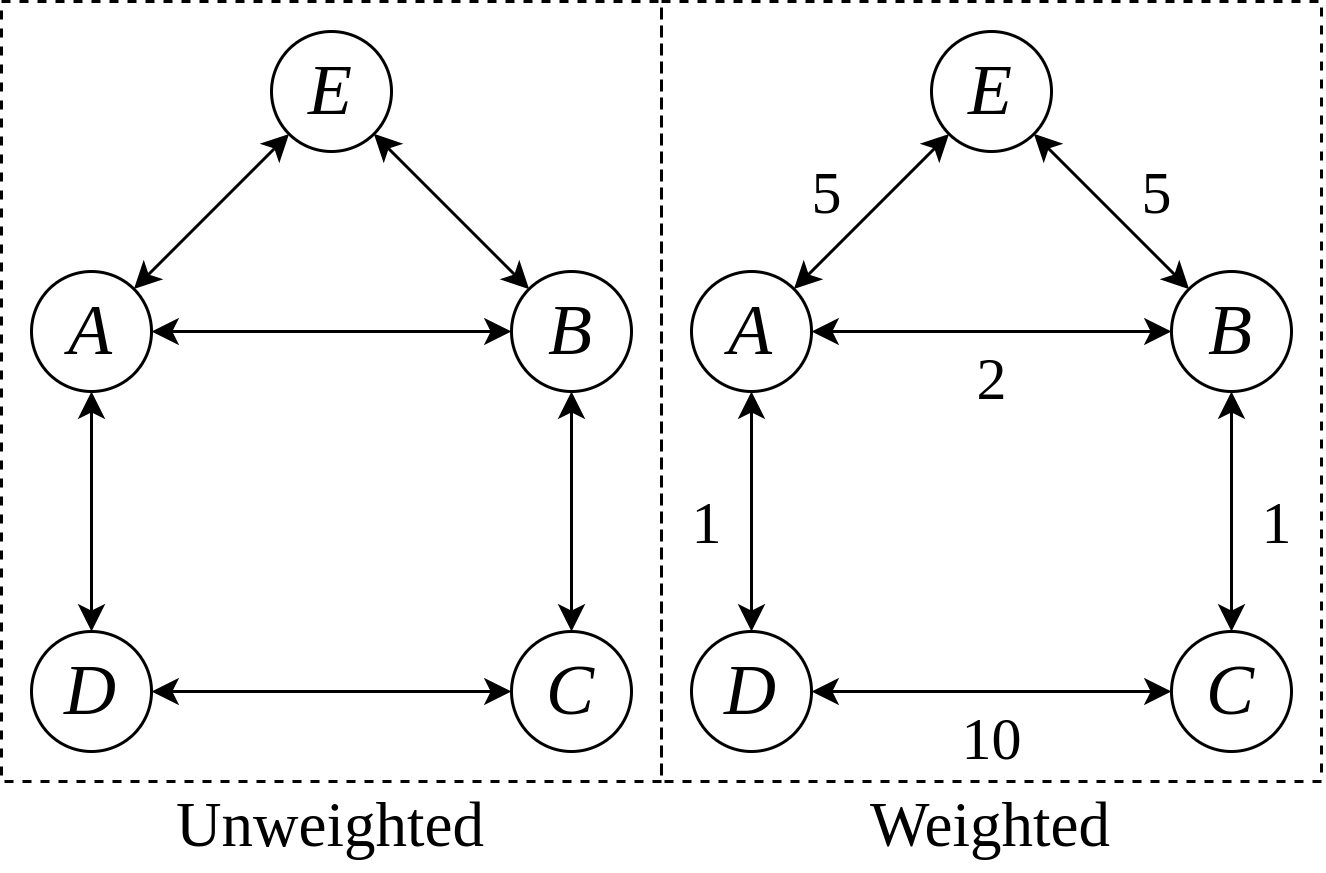
\includegraphics[width = .5\linewidth]{figs/simple_graph.png}
	\caption{Simple example undirected graph unweighted and weighted isomorphs}
	\label{fig:simple_graph}
\end{figure}

\begin{table}[H]
	\centering
	\caption{Centrality for simple undirected and unweighted example graph}
	\label{tab:unweighted_centrality}
	\begin{tabular}{|C{.2\linewidth}|C{.2\linewidth}|C{.2\linewidth}|C{.2\linewidth}|C{.2\linewidth}|}
		\hline Node & Degree Centrality & Betweenness Centrality & Closeness Centrality & Information Centrality \\
		\hline A & 0.75 & 0.25 & 0.8 & 0.355 \\
		\hline B & 0.75 & 0.25 & 0.8 & 0.355 \\
		\hline C & 0.5 & 0.083 & 0.667 & 0.282 \\
		\hline D & 0.5 & 0.083 & 0.667 & 0.282 \\
		\hline E & 0.5 & 0 & 0.667 & 0.275 \\
		\hline
	\end{tabular}
\end{table}

\begin{table}[H]
	\centering
	\caption{Centrality for simple undirected and weighted example graph}
	\label{tab:weighted_centrality}
	\begin{tabular}{|C{.2\linewidth}|C{.2\linewidth}|C{.2\linewidth}|C{.2\linewidth}|C{.2\linewidth}|}
		\hline Node & Degree Centrality & Betweenness Centrality & Closeness Centrality & Information Centrality \\
		\hline A & 0.75 & 0.5 & 0.364 & 0.667 \\
		\hline B & 0.75 & 0.5 & 0.364 & 0.667 \\
		\hline C & 0.5 & 0 & 0.286 & 0.535 \\
		\hline D & 0.5 & 0 & 0.286 & 0.535 \\
		\hline E & 0.5 & 0 & 0.182 & 0.646 \\
		\hline
	\end{tabular}
\end{table}

Concerning the isomorphs in Figure \ref{fig:simple_graph}, intuition would say that nodes $A$ and $B$ are most central and this is supported by all centrality measures presented. The principle effects of considering edge weights are that the shortest paths between $C$ and $D$ no longer utilize $(C, D)$, all shortest paths include $A$ or $B$, and 3 include $(A, B)$. The differences are not attested to by degree centrality which is identical among isomorphs. The increased reliance of the network on $A$ and $B$ is reflected in the remaining centrality metrics. It is worth noting that, although the relative closeness centrality of $A$ and $B$ increased to reflect their greater importance, the gross values for $A$ and $B$ decreased due to the greater-than-one edge weights. The lower diversity of paths for the weighted graph is also reflected in the higher information centrality values for the nodes.

Ultimately, for a given application, some definition of centrality must be chosen. Ultimately, some metric must be computed for whole networks or subnetworks of interest. For transportation network resilience betweenness and information centrality are particularly relevant. It is straightforward that removing a node which is highly central by either definition will cause a shift in traffic which results in worse overall performance. The difference between the measures is exemplified by node $E$. $E$ has the same degree as $C$ and $D$ but is directly connected to the high degree nodes $A$ and $B$ where $C$ and $D$ are connected to a high degree node and each-other. For the weighted graph, nodes $C$, $D$, and $E$ occur on no shortest paths and are, thus, equal from a betweenness perspective. Information centrality, however, captures the subtle difference that after leaving $E$ it will be known if $A$ or $B$ is next. Thus the information gained through visiting $E$ is higher than that gained by visiting $C$ or $D$ because someone \textit{could} traverse $(C, D)$. In other words, \textbf{betweenness centrality is descriptive while information centrality is fundamental}. Philosophically a network with generally low and evenly distributed information centrality at all nodes will be quite redundant increasing its resilience while its efficiency and vice versa. A corollary is that network resilience can be optimized for via entropy maximization. Information centrality has the additional advantage of being less costly to compute.

In order to apply information centrality to \gls{bev} transportation a slight reformulation is required and this measure is herein called \gls{rsic}. The elements of the $B$ matrix for \gls{rsic} are

\begin{align}
	b_{ij} = \begin{cases}
		1 & (i, j) \not\in E \\
		1 & \eta(i, j)>l \\
		1 - \eta(i, j) & otherwise
	\end{cases}\\
	b_{ii} = 1 + \sum_{(i, j) \in E_i} \eta(i, j)
\end{align}

where $l$ is vehicle range. This modification reflects the inadmissibility of edges greater than vehicle range. \gls{rsic} for node $i$ is calculated as in \eqref{eq:information_centrality}. \gls{rsbc} is the equivalent of betweenness centrality for vehicles and is computed as in \eqref{eq:betweenness_centrality} also neglecting those edges which exceed vehicle range. Figure \ref{fig:bev_centrality} shows \gls{rsic} and \gls{rsbc} for the randomly generated transportation system example.

\begin{figure}[H]
	\centering
	\begin{subfigure}[t]{.5\linewidth}
		\centering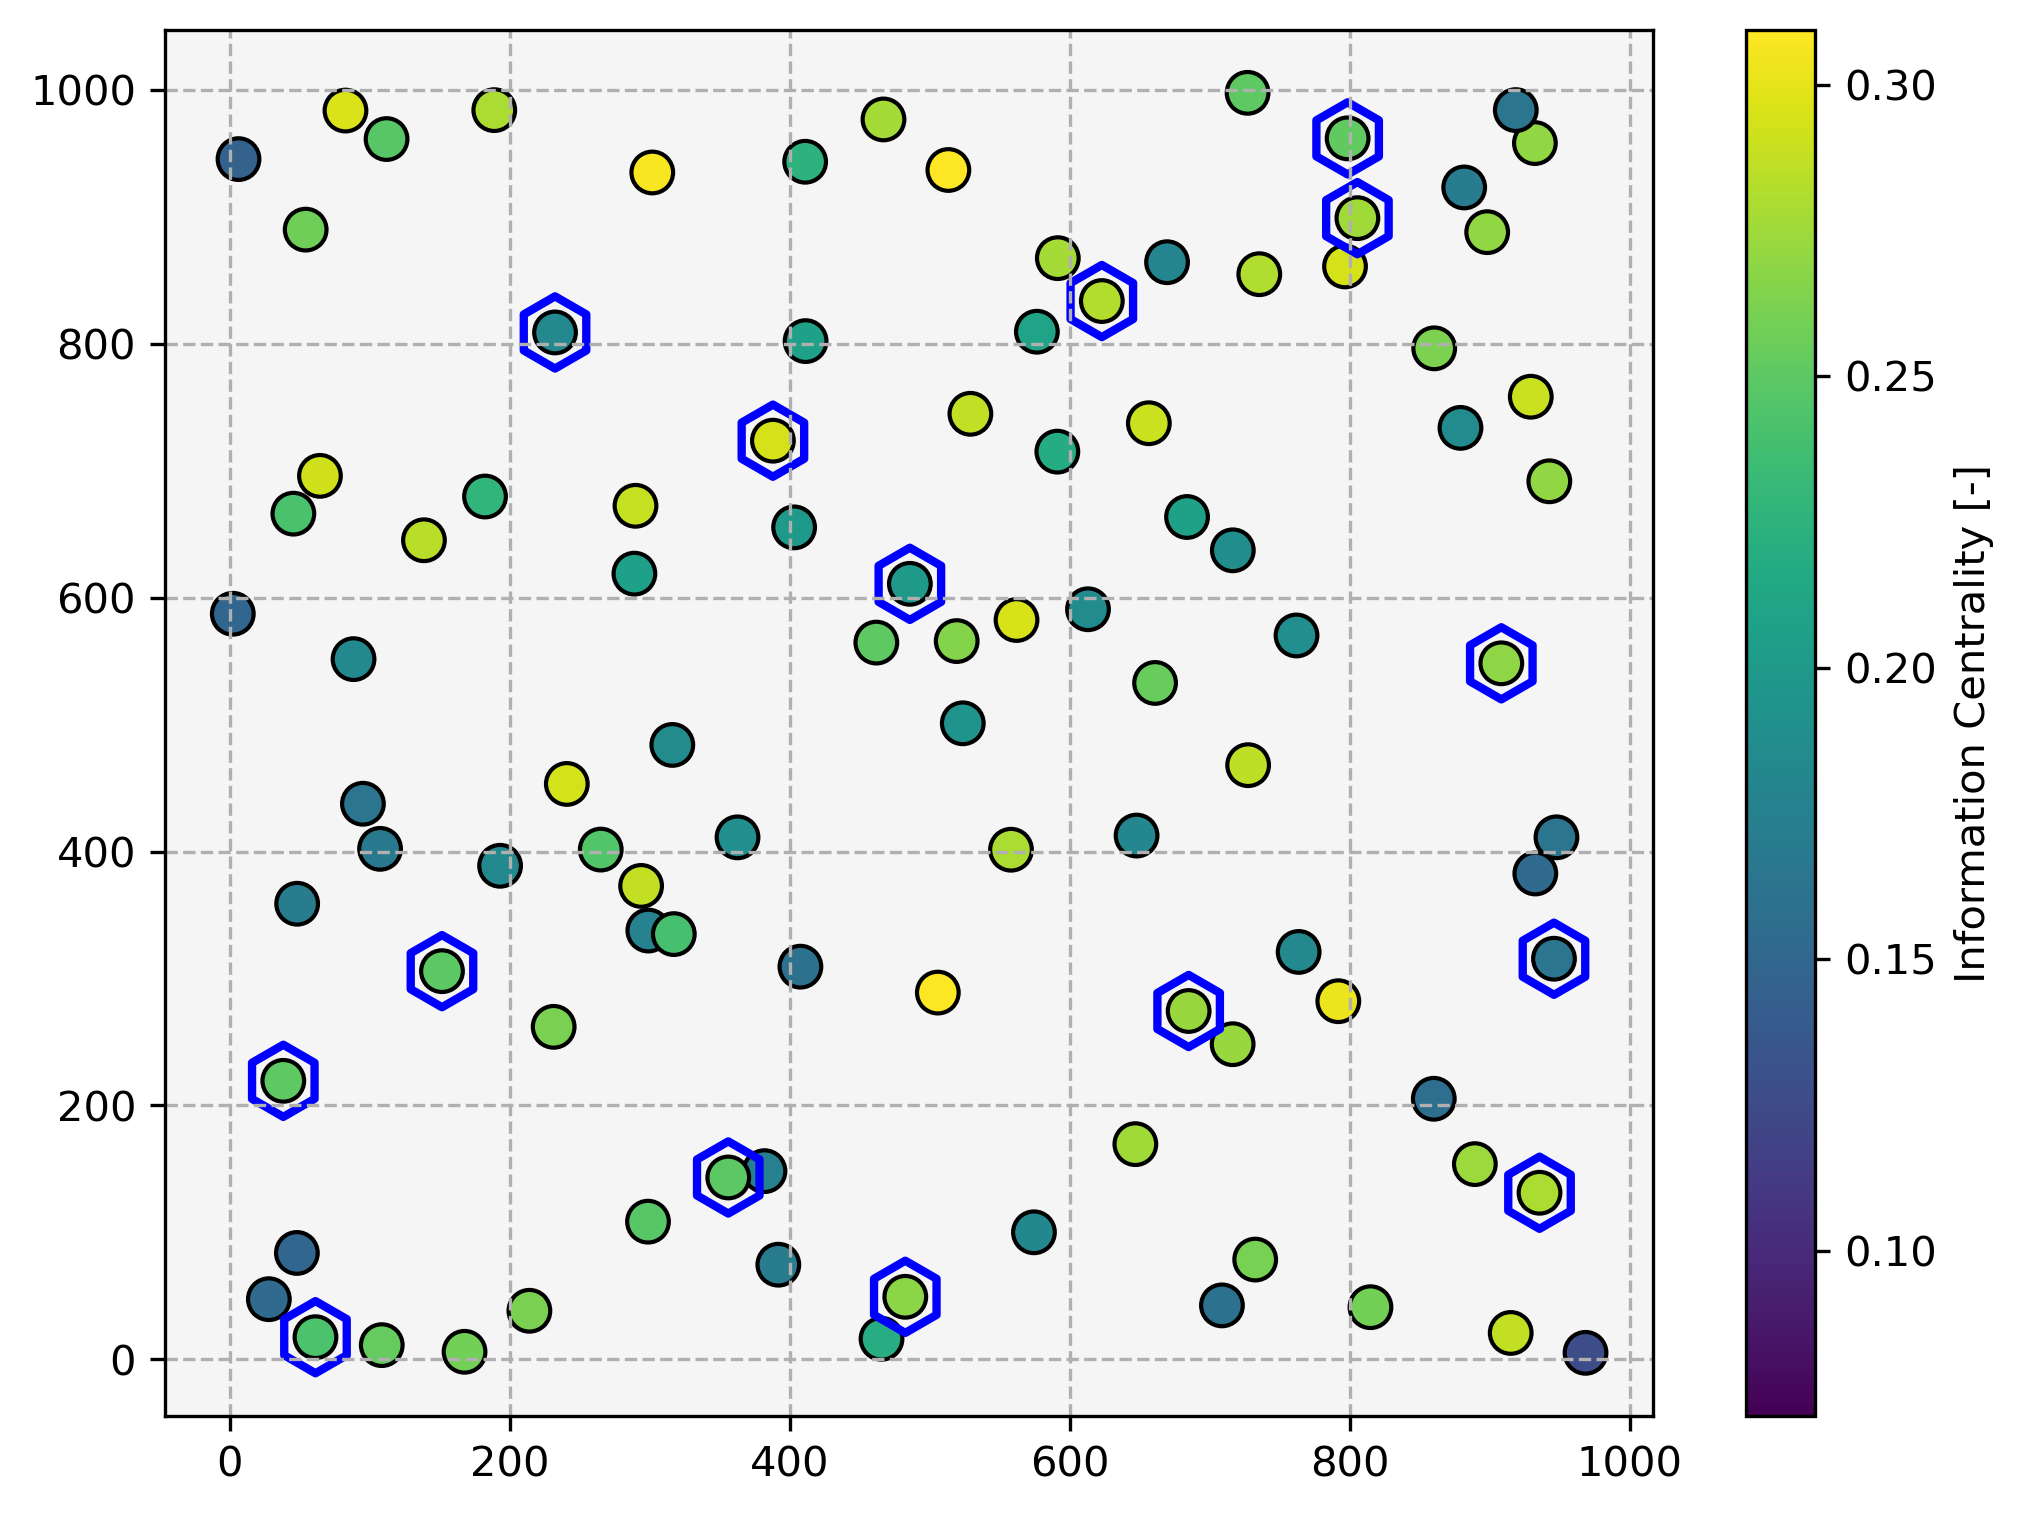
\includegraphics[width = \linewidth]{figs/information_centrality.png}
		\captionsetup{width=.8\linewidth}
		\caption{Information Centrality}
	\end{subfigure}%
	\begin{subfigure}[t]{.5\linewidth}
		\centering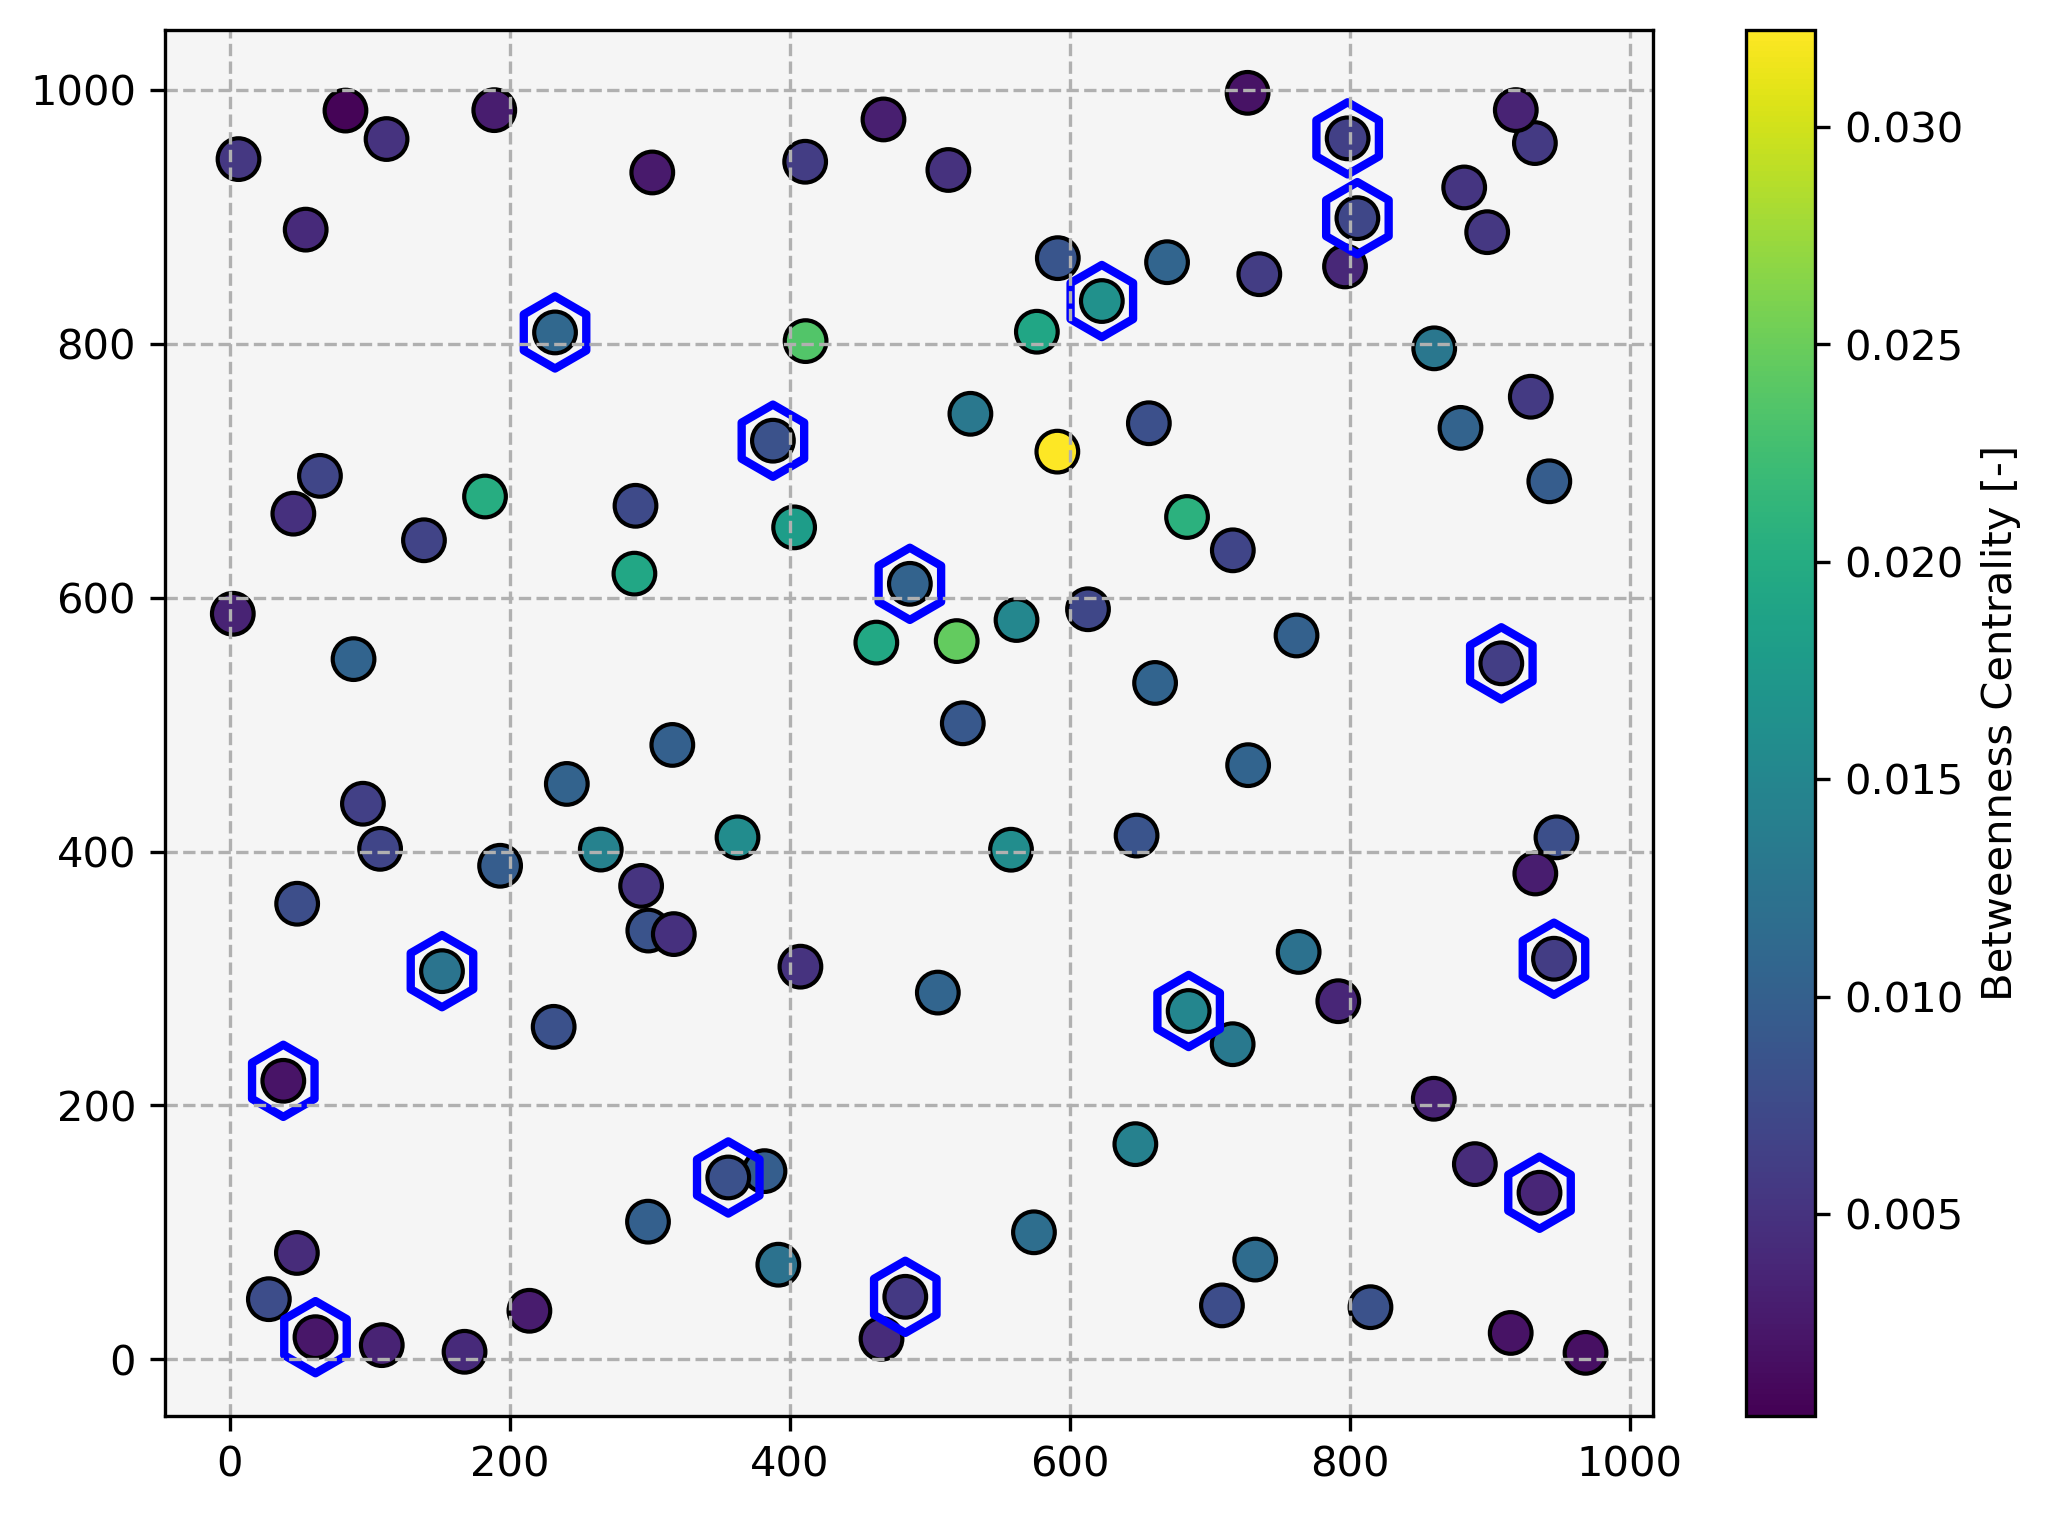
\includegraphics[width = \linewidth]{figs/betweenness_centrality.png}
		\captionsetup{width=.8\linewidth}
		\caption{Betweenness Centrality}
	\end{subfigure}
	\caption{Centrality measures for example transportation network.}
	\label{fig:bev_centrality}
\end{figure}

Information \gls{rsic} is likely the more useful metric for the above scenario. \gls{rsbc} is more heavily influenced by geometric proximity and thus, minimizing \gls{rsbc} will be less useful for increasing resilience. \gls{rsic} minimization could be done on the basis of gross or average \gls{rsic} or on the basis of inequality (Gini coefficient).